\section{Schema E-R + business rules }
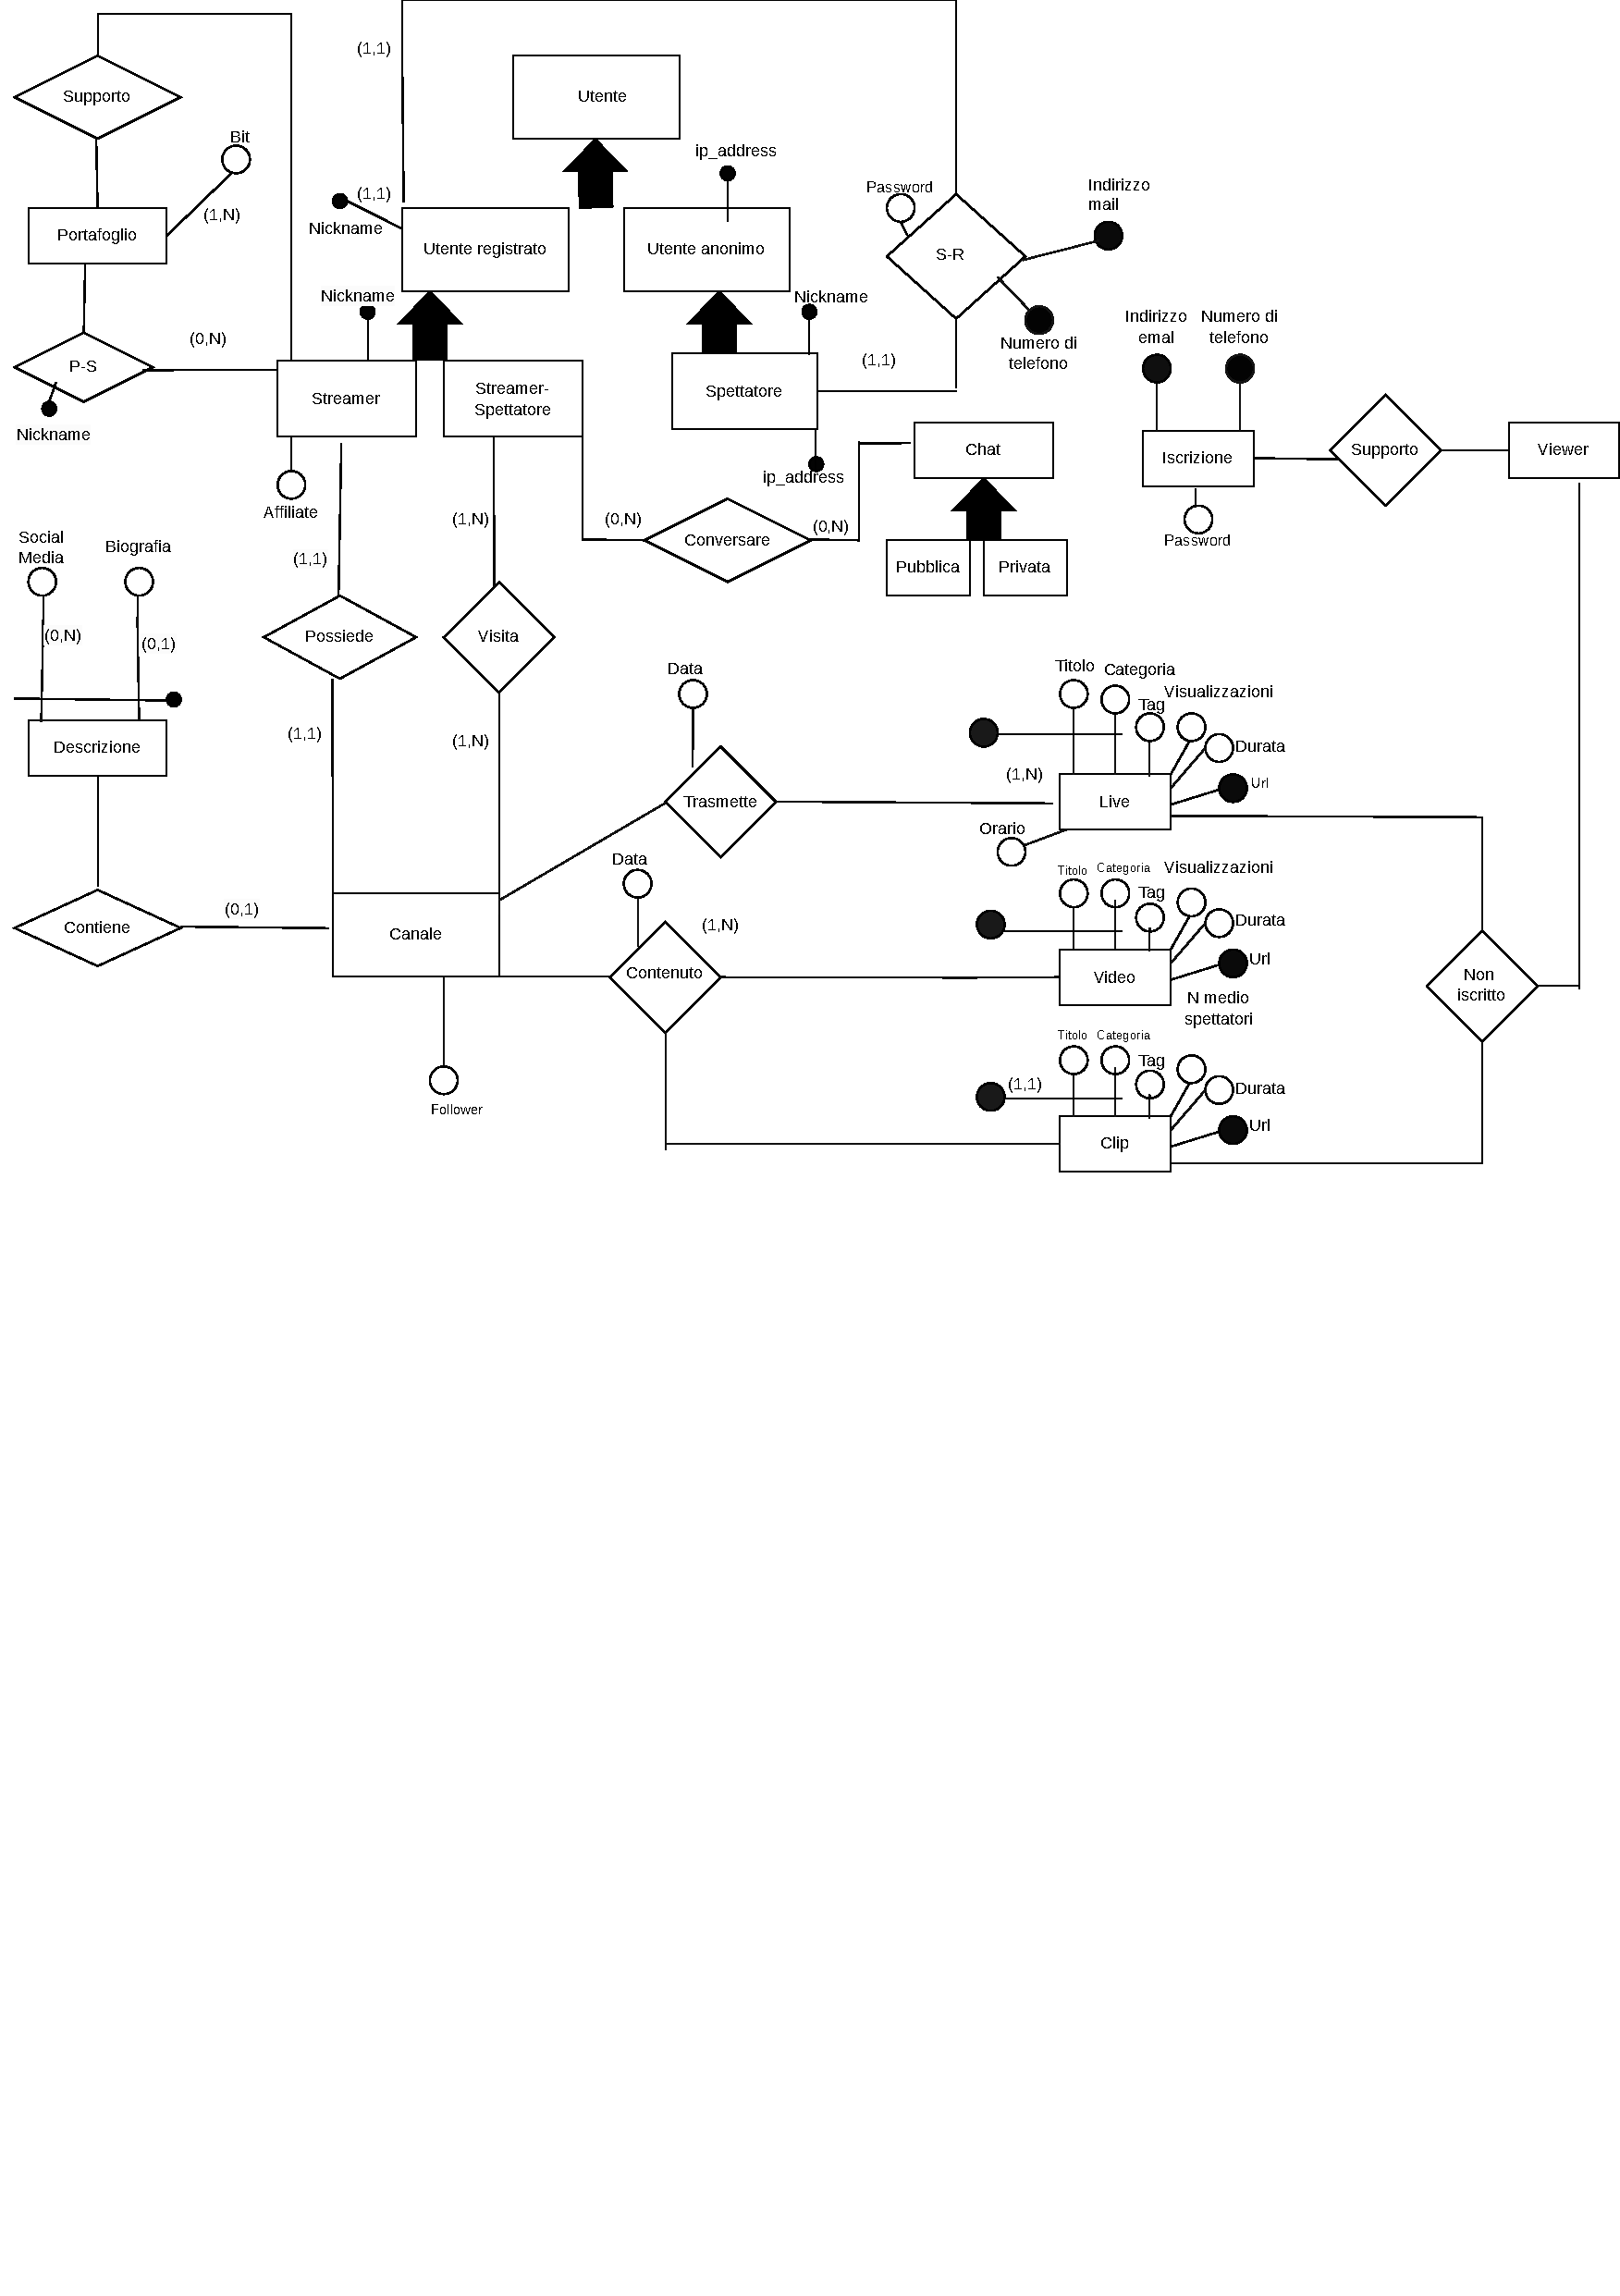
\includegraphics[width=\textwidth]{resources/schema_e-r.pdf}
\subsection{Vincoli di integrità}
\begin{itemize}
    \item I video sono degli estratti di live passate.
    \item Le clip sono dei video di breve durata.
    \item I bit può essere acquistato nella piattaforma.
    \item Un utente per registrarsi sulla piattaforma deve fornire indirizzo email o numero di telefono.
    \begin{itemize}
        \item Un utente anonimo può guardare la live trasmessa dallo streamer ma non può interagire con esso. 
    \end{itemize}
    \item All'interno del canale sono presenti live passate ma anche la trasmissione in tempo reale di una eventuale live in atto.
    \item Ogni contenuto all'interno della piattaforma è identificato con un indirizzo \textbf{Url}.
    \item 
        \item Se uno \textit{streamer} rispetta i \textit{parametri di performance} può diventare \textit{affiliate}.
        \item Il portafoglio è costituito da \textit{bit}, con i quali il \textbf{follower} può supportare lo streamer
        \item Il viewer non può supportare lo streamer.
        \item La chat permette agli utenti di comunicare l'uno con l'altro sia pubblicamente sia privatamente.
        \item Il nome del canale è lo stesso nome che l'utente inserisce durante la registrazione alla piattaforma.
        \item All'interno del canale è presente una biografia. 
        \item All'interno del canale è presente una lista di link ad altri social media.
\end{itemize}